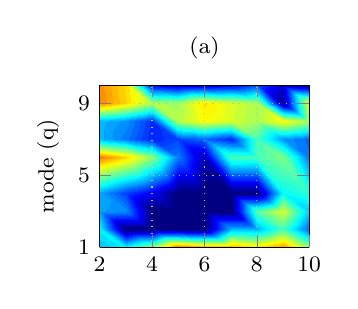
\begin{tikzpicture}
\begin{axis}
[
width=0.35\textwidth,
height=0.3\textwidth,
style={font=\footnotesize},
grid=major,
grid style={dotted},
align=center,
%xlabel={tensor order},
ylabel={mode (q)},
title={(a)}, % tlib{\scriptsize (bgemm,subtensor)}
scaled ticks=false,
zlabel={Performance [TFlops/s]},
view={0}{90}, 
ytick={1,5,9},
xtick={2,4,6,8,10},
%yticklabels={32,256,512,768,1024}, 
xmin=2, xmax=10,
ymin=1, ymax=10,
try min ticks=8,
zmin=500, zmax=1100,
point meta min=500, point meta max=1100,
colormap/jet, 
colormap access=piecewise const,
]
\addplot3[contour filled={number=50}]
coordinates{
(2.000,1.000,688.655) (2.000,2.000,721.564) (2.000,3.000,669.598) (2.000,4.000,673.295) (2.000,6.000,951.352) (2.000,7.000,683.991) (2.000,8.000,686.396) (2.000,9.000,944.347) (2.000,10.000,938.327) 

(3.000,1.000,724.016) (3.000,2.000,358.459) (3.000,3.000,661.743) (3.000,4.000,614.798) (3.000,6.000,899.354) (3.000,7.000,649.071) (3.000,8.000,662.775) (3.000,9.000,897.004) (3.000,10.000,892.134) 

(4.000,1.000,812.593) (4.000,2.000,336.129) (4.000,3.000,333.389) (4.000,4.000,570.847) (4.000,6.000,810.443) (4.000,7.000,598.168) (4.000,8.000,604.120) (4.000,9.000,826.964) (4.000,10.000,576.327) 

(5.000,1.000,959.382) (5.000,2.000,313.810) (5.000,3.000,332.101) (5.000,4.000,375.380) (5.000,6.000,651.385) (5.000,7.000,618.244) (5.000,8.000,831.026) (5.000,9.000,818.826) (5.000,10.000,548.918) 

(6.000,1.000,928.709) (6.000,2.000,332.294) (6.000,3.000,381.673) (6.000,4.000,398.248) (6.000,6.000,538.255) (6.000,7.000,638.543) (6.000,8.000,873.527) (6.000,9.000,888.014) (6.000,10.000,554.649) 

(7.000,1.000,921.397) (7.000,2.000,684.634) (7.000,3.000,338.925) (7.000,4.000,384.162) (7.000,6.000,769.746) (7.000,7.000,599.565) (7.000,8.000,849.478) (7.000,9.000,853.490) (7.000,10.000,571.199) 

(8.000,1.000,889.512) (8.000,2.000,681.510) (8.000,3.000,778.088) (8.000,4.000,384.863) (8.000,6.000,766.658) (8.000,7.000,766.801) (8.000,8.000,821.863) (8.000,9.000,824.276) (8.000,10.000,624.293) 

(9.000,1.000,937.702) (9.000,2.000,767.676) (9.000,3.000,850.378) (9.000,4.000,729.556) (9.000,6.000,798.204) (9.000,7.000,668.046) (9.000,8.000,875.833) (9.000,9.000,517.109) (9.000,10.000,549.323) 

(10.000,1.000,807.944) (10.000,2.000,637.553) (10.000,3.000,696.294) (10.000,4.000,749.176) (10.000,6.000,645.879) (10.000,7.000,638.822) (10.000,8.000,822.516) (10.000,9.000,861.514) (10.000,10.000,512.969) 
};
\end{axis}
\end{tikzpicture}
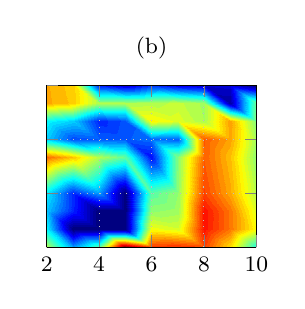
\begin{tikzpicture}
\begin{axis}%
[%
width=0.35\textwidth,
height=0.3\textwidth,
style={font=\footnotesize},
grid=major,
grid style={dotted},
align=center,
%xlabel={tensor order},
title={(b)}, % title={tlib{\scriptsize <ompfor,slice>}},
scaled ticks=false,
zlabel={Performance [TFlops/s]},
view={0}{90},
yticklabel=\empty,
ytick={1,4,7,10},
xtick={2,4,6,8,10},
xmin=2, xmax=10,
ymin=1, ymax=10,
try min ticks=8,
zmin=500, zmax=1100,
point meta min=500, point meta max=1100,
colormap/jet, 
colormap access=piecewise const,
]
\addplot3[contour filled={number=50}]
coordinates{
(2.000,1.000,829.067) (2.000,2.000,720.556) (2.000,3.000,691.297) (2.000,4.000,714.721) (2.000,6.000,958.952) (2.000,7.000,695.849) (2.000,8.000,725.682) (2.000,9.000,923.561) (2.000,10.000,921.564) 

(3.000,1.000,671.586) (3.000,2.000,127.615) (3.000,3.000,598.752) (3.000,4.000,602.496) (3.000,6.000,906.916) (3.000,7.000,621.776) (3.000,8.000,699.517) (3.000,9.000,904.113) (3.000,10.000,900.147) 

(4.000,1.000,780.280) (4.000,2.000,251.473) (4.000,3.000,248.999) (4.000,4.000,669.714) (4.000,6.000,828.702) (4.000,7.000,632.583) (4.000,8.000,599.336) (4.000,9.000,825.843) (4.000,10.000,590.894) 

(5.000,1.000,1148.593) (5.000,2.000,480.197) (5.000,3.000,475.819) (5.000,4.000,462.756) (5.000,6.000,782.908) (5.000,7.000,629.366) (5.000,8.000,624.551) (5.000,9.000,826.017) (5.000,10.000,550.087) 

(6.000,1.000,987.913) (6.000,2.000,867.653) (6.000,3.000,809.609) (6.000,4.000,778.857) (6.000,6.000,584.026) (6.000,7.000,642.762) (6.000,8.000,877.038) (6.000,9.000,828.948) (6.000,10.000,602.083) 

(7.000,1.000,997.606) (7.000,2.000,851.140) (7.000,3.000,817.599) (7.000,4.000,812.076) (7.000,6.000,806.244) (7.000,7.000,632.070) (7.000,8.000,855.686) (7.000,9.000,840.731) (7.000,10.000,565.177) 

(8.000,1.000,982.270) (8.000,2.000,1011.196) (8.000,3.000,1012.914) (8.000,4.000,981.783) (8.000,6.000,966.488) (8.000,7.000,968.924) (8.000,8.000,824.110) (8.000,9.000,820.097) (8.000,10.000,549.434) 

(9.000,1.000,892.197) (9.000,2.000,953.453) (9.000,3.000,952.376) (9.000,4.000,923.914) (9.000,6.000,910.070) (9.000,7.000,926.784) (9.000,8.000,928.569) (9.000,9.000,524.263) (9.000,10.000,554.261) 

(10.000,1.000,743.042) (10.000,2.000,871.808) (10.000,3.000,854.549) (10.000,4.000,831.029) (10.000,6.000,807.998) (10.000,7.000,819.963) (10.000,8.000,801.759) (10.000,9.000,793.293) (10.000,10.000,467.283) 
};
\end{axis}
\end{tikzpicture}
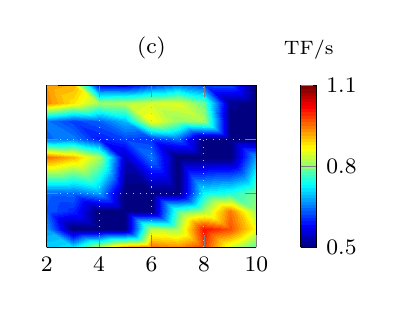
\begin{tikzpicture}
\begin{axis}
[
width=0.35\textwidth,
height=0.3\textwidth,
style={font=\footnotesize},
grid=major,
grid style={dotted},
align=center,
%xlabel={tensor order},
title={(c)}, % title={tlib{\scriptsize <ompfor,subtensor>}},
scaled ticks=false,
yticklabel=\empty,
ytick={1,4,7,10},
xtick={2,4,6,8,10},
zlabel={Performance [TFlops/s]},
view={0}{90}, 
xmin=2, xmax=10,  
ymin=1, ymax=10,
try min ticks=8,
zmin=500, zmax=1100,
point meta min=500, point meta max=1100,
colormap/jet, 
colormap access=piecewise const,
colorbar sampled,
colorbar/width=0.2cm,
colorbar style={
	point meta min=500, point meta max=1100,
	samples=50,
	font=\footnotesize,
	ytick={500,800,1100},
	yticklabels={0.5,0.8,1.1},
	title={\scriptsize TF/s},
}
]
\addplot3[contour filled={number=50}]
coordinates{
(2.000,1.000,701.148) (2.000,2.000,668.348) (2.000,3.000,629.823) (2.000,4.000,636.757) (2.000,6.000,958.671) (2.000,7.000,640.769) (2.000,8.000,646.998) (2.000,9.000,941.899) (2.000,10.000,930.142) 

(3.000,1.000,713.250) (3.000,2.000,126.667) (3.000,3.000,601.581) (3.000,4.000,638.836) (3.000,6.000,916.366) (3.000,7.000,653.609) (3.000,8.000,613.576) (3.000,9.000,888.591) (3.000,10.000,917.722) 

(4.000,1.000,834.786) (4.000,2.000,251.316) (4.000,3.000,129.291) (4.000,4.000,674.193) (4.000,6.000,824.425) (4.000,7.000,592.512) (4.000,8.000,634.149) (4.000,9.000,817.756) (4.000,10.000,572.485) 

(5.000,1.000,928.389) (5.000,2.000,482.929) (5.000,3.000,247.467) (5.000,4.000,126.153) (5.000,6.000,544.270) (5.000,7.000,617.168) (5.000,8.000,687.186) (5.000,9.000,829.083) (5.000,10.000,568.107) 

(6.000,1.000,956.421) (6.000,2.000,834.518) (6.000,3.000,448.775) (6.000,4.000,245.940) (6.000,6.000,649.715) (6.000,7.000,607.233) (6.000,8.000,874.057) (6.000,9.000,849.136) (6.000,10.000,615.486) 

(7.000,1.000,938.567) (7.000,2.000,824.455) (7.000,3.000,775.559) (7.000,4.000,463.045) (7.000,6.000,124.761) (7.000,7.000,635.238) (7.000,8.000,811.691) (7.000,9.000,856.776) (7.000,10.000,653.732) 

(8.000,1.000,986.503) (8.000,2.000,1014.924) (8.000,3.000,820.959) (8.000,4.000,725.559) (8.000,6.000,241.433) (8.000,7.000,123.843) (8.000,8.000,825.934) (8.000,9.000,786.079) (8.000,10.000,618.081) 

(9.000,1.000,850.595) (9.000,2.000,976.051) (9.000,3.000,952.992) (9.000,4.000,743.869) (9.000,6.000,453.796) (9.000,7.000,237.399) (9.000,8.000,121.051) (9.000,9.000,517.079) (9.000,10.000,623.085) 

(10.000,1.000,770.743) (10.000,2.000,867.312) (10.000,3.000,814.667) (10.000,4.000,792.499) (10.000,6.000,674.668) (10.000,7.000,406.107) (10.000,8.000,214.465) (10.000,9.000,109.557) (10.000,10.000,435.371) 	
};
\end{axis}
\end{tikzpicture}


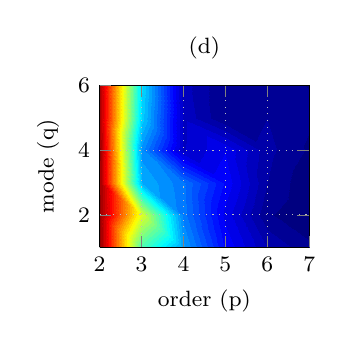
\begin{tikzpicture}
\begin{axis}
[
width=0.35\textwidth,
height=0.3\textwidth,
style={font=\footnotesize},
grid=major,
grid style={dotted},
align=center,
xlabel={order (p)},
ylabel={mode (q)},
title={(d)}, %title={tlib<bgemm,subtensor>},
scaled ticks=false,
zlabel={Performance [TFlops/s]},
view={0}{90}, 
ytick={2,4,6},
xtick={2,3,4,5,6,7},
%yticklabels={32,256,512,768,1024}, 
xmin=2, xmax=7,
ymin=1, ymax=6,
zmin=50, zmax=1700,
point meta min=50, point meta max=1700,
colormap/jet, 
colormap access=piecewise const,
]
\addplot3[contour filled={number=50}]
coordinates{
(2.000,1.000,1647.736) (2.000,2.000,1639.687) (2.000,3.000,1630.864) (2.000,4.000,1635.471) (2.000,5.000,1612.667) (2.000,6.000,1609.485) 

(3.000,1.000,788.257) (3.000,2.000,1020.523) (3.000,3.000,546.272) (3.000,4.000,493.357) (3.000,5.000,596.070) (3.000,6.000,615.648) 

(4.000,1.000,523.762) (4.000,2.000,466.629) (4.000,3.000,455.783) (4.000,4.000,177.272) (4.000,5.000,176.459) (4.000,6.000,165.932) 

(5.000,1.000,277.077) (5.000,2.000,236.257) (5.000,3.000,274.769) (5.000,4.000,245.515) (5.000,5.000,84.956) (5.000,6.000,84.735) 

(6.000,1.000,148.311) (6.000,2.000,89.238) (6.000,3.000,116.228) (6.000,4.000,127.542) (6.000,5.000,115.673) (6.000,6.000,91.095) 

(7.000,1.000,92.213) (7.000,2.000,22.391) (7.000,3.000,54.655) (7.000,4.000,78.167) (7.000,5.000,87.540) (7.000,6.000,82.204) 
};
\end{axis}
\end{tikzpicture}
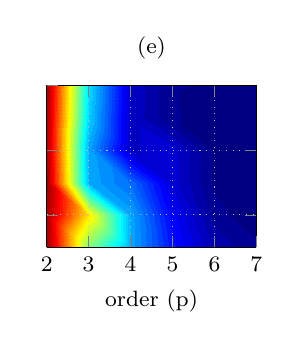
\begin{tikzpicture}
\begin{axis}%
[%
width=0.35\textwidth,
height=0.3\textwidth,
style={font=\footnotesize},
grid=major,
grid style={dotted},
align=center,
xlabel={order (p)},
title={(e)}, %title={tlib<tgemm,slice,all>},
scaled ticks=false,
view={0}{90},
yticklabel=\empty,
ytick={2,4,6},
xtick={2,3,4,5,6,7},
xmin=2, xmax=7,
ymin=1, ymax=6,
zmin=50, zmax=1700,
point meta min=50, point meta max=1700,
colormap/jet, 
colormap access=piecewise const,
]
\addplot3[contour filled={number=50}]
coordinates{
(2.000,1.000,1638.950) (2.000,2.000,1616.152) (2.000,3.000,1638.577) (2.000,4.000,1616.161) (2.000,5.000,1618.750) (2.000,6.000,1630.884) 

(3.000,1.000,877.821) (3.000,2.000,1107.668) (3.000,3.000,540.389) (3.000,4.000,527.151) (3.000,5.000,595.677) (3.000,6.000,618.358) 

(4.000,1.000,534.527) (4.000,2.000,529.750) (4.000,3.000,438.960) (4.000,4.000,176.985) (4.000,5.000,176.867) (4.000,6.000,180.903) 

(5.000,1.000,294.534) (5.000,2.000,260.419) (5.000,3.000,200.560) (5.000,4.000,200.048) (5.000,5.000,85.195) (5.000,6.000,84.598) 

(6.000,1.000,143.466) (6.000,2.000,103.224) (6.000,3.000,74.911) (6.000,4.000,75.566) (6.000,5.000,75.502) (6.000,6.000,80.650) 

(7.000,1.000,91.477) (7.000,2.000,24.796) (7.000,3.000,19.944) (7.000,4.000,19.933) (7.000,5.000,19.941) (7.000,6.000,19.877) 
};
\end{axis}
\end{tikzpicture}
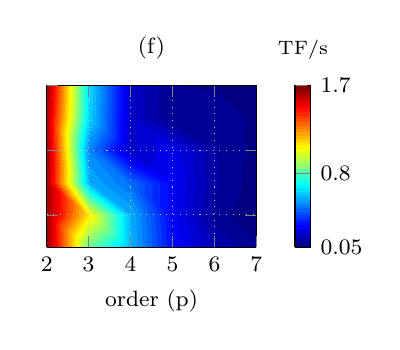
\begin{tikzpicture}
\begin{axis}
[
width=0.35\textwidth,
height=0.3\textwidth,
style={font=\footnotesize},
grid=major,
grid style={dotted},
align=center,
xlabel={order (p)},
title={(f)}, %title={tlib<ompfor,slice,all>},
scaled ticks=false,
view={0}{90},
yticklabel=\empty,
ytick={2,4,6},
xtick={2,3,4,5,6,7},
xmin=2, xmax=7,
ymin=1, ymax=6,
zmin=50, zmax=1700,
point meta min=50, point meta max=1700,
colormap/jet, 
colormap access=piecewise const,
colorbar sampled,
colorbar/width=0.2cm,
colorbar style={
	%point meta min=-2e-3, %neu     % Beginn Colorbar, beachte yticks min
	%point meta max=2e-3, %neu      % Ende Colorbar, beachte yticks max
	%scaled y ticks = false,
	point meta min=50, point meta max=1700,
	samples=50,
	font=\footnotesize,		
	ytick={50,800,1700},
	yticklabels={0.05,0.8,1.7},
	title={\scriptsize TF/s},
}
]
\addplot3[contour filled={number=50}]
coordinates{
(2.000,1.000,1646.678) (2.000,2.000,1630.607) (2.000,3.000,1626.251) (2.000,4.000,1630.192) (2.000,5.000,1601.485) (2.000,6.000,1639.470) 

(3.000,1.000,839.726) (3.000,2.000,1102.508) (3.000,3.000,548.776) (3.000,4.000,478.249) (3.000,5.000,606.091) (3.000,6.000,618.214) 

(4.000,1.000,545.963) (4.000,2.000,544.155) (4.000,3.000,439.090) (4.000,4.000,173.662) (4.000,5.000,178.016) (4.000,6.000,180.045) 

(5.000,1.000,279.095) (5.000,2.000,259.332) (5.000,3.000,262.099) (5.000,4.000,239.972) (5.000,5.000,85.286) (5.000,6.000,84.263) 

(6.000,1.000,147.667) (6.000,2.000,103.102) (6.000,3.000,122.330) (6.000,4.000,119.210) (6.000,5.000,103.976) (6.000,6.000,78.724) 

(7.000,1.000,90.412) (7.000,2.000,24.888) (7.000,3.000,64.061) (7.000,4.000,72.989) (7.000,5.000,76.168) (7.000,6.000,60.167) 	
};
\end{axis}
\end{tikzpicture}